\documentclass{article}

% Official NeurIPS 2026 style, loaded with NO options. This is deliberate and
% venue-neutral, so one PDF can go to more than one workshop:
%   * `final' and `preprint' are omitted, which the call for papers requires --
%     \if@anonymous defaults TRUE, so the anonymous author block still applies;
%   * `dblblindworkshop' is also omitted. In this style file \if@workshop is read
%     in exactly one place (neurips_2026.sty:401), the footer notice, and gates
%     nothing else -- not anonymity. With it, the footer names one workshop;
%     without it, the footer reads "Submitted to 40th Conference on Neural
%     Information Processing Systems (NeurIPS 2026). Do not distribute."
% SIMBIOCHEM II asks only that `final' and `preprint' be omitted, does not
% require its name in the footer, and is non-archival and explicitly welcomes
% work "currently under review elsewhere".
\usepackage{neurips_2026}

\usepackage[utf8]{inputenc}
\usepackage[T1]{fontenc}
\usepackage[hidelinks]{hyperref}
\usepackage{url}
\usepackage{doi}          % renders the bibliography's doi field as a hyperlink
\usepackage{booktabs}
\usepackage{amsfonts}
\usepackage{amsmath}
\usepackage{amssymb}
\usepackage{nicefrac}
\usepackage{microtype}
\usepackage{graphicx}
\usepackage{xcolor}

% Every number below comes from paper/macros.tex, regenerated from results/raw by
% analysis/tables.py. Do not write a literal result into this file.
% Generated by analysis/tables.py -- do not edit by hand.
\newcommand{\fsCostIntercept}{10.38}
\newcommand{\fsCostSlope}{11.78}
\newcommand{\fsHaarRecallKTwo}{0.450}
\newcommand{\fsHaarSpearmanKTwo}{0.676}
\newcommand{\fsHaarRecallKThree}{0.529}
\newcommand{\fsHaarSpearmanKThree}{0.781}
\newcommand{\fsHaarRecallKFour}{0.619}
\newcommand{\fsHaarSpearmanKFour}{0.859}
\newcommand{\fsHaarRecallKFive}{0.717}
\newcommand{\fsHaarSpearmanKFive}{0.916}
\newcommand{\fsHaarRecallKSix}{0.834}
\newcommand{\fsHaarSpearmanKSix}{0.962}
\newcommand{\fsHeadSubRecallKThree}{0.477}
\newcommand{\fsGaussRecallKThree}{0.304}
\newcommand{\fsTotalKThreeBOne}{1.83}
\newcommand{\fsTotalKTwoBOne}{2.31}
\newcommand{\fsIncrKThreeBOne}{2.34}
\newcommand{\fsIncrKTwoBOne}{3.51}
\newcommand{\fsTotalKThreeBSixtyFour}{1.87}
\newcommand{\fsTotalKTwoBSixtyFour}{2.39}
\newcommand{\fsIncrKThreeBSixtyFour}{2.33}
\newcommand{\fsIncrKTwoBSixtyFour}{3.51}
\newcommand{\fsGateSkipThreeBPA}{0.857}
\newcommand{\fsGateRecallThreeBPA}{0.983}
\newcommand{\fsGateSpeedupThreeBPA}{1.38}
\newcommand{\fsGateSkipEthanol}{0.777}
\newcommand{\fsGateRecallEthanol}{0.976}
\newcommand{\fsGateSpeedupEthanol}{1.32}
\newcommand{\fsGateSkipAspirin}{0.758}
\newcommand{\fsGateRecallAspirin}{0.993}
\newcommand{\fsGateSpeedupAspirin}{1.30}
\newcommand{\fsGateSkipAzobenzene}{0.845}
\newcommand{\fsGateRecallAzobenzene}{0.971}
\newcommand{\fsGateSpeedupAzobenzene}{1.37}
\newcommand{\fsNBoot}{10,000}
\newcommand{\fsHaarRecallKTwoCI}{[0.414, 0.479]}
\newcommand{\fsHaarSpearmanKTwoCI}{[0.661, 0.689]}
\newcommand{\fsHaarRecallKThreeCI}{[0.490, 0.566]}
\newcommand{\fsHaarSpearmanKThreeCI}{[0.768, 0.792]}
\newcommand{\fsHaarRecallKFourCI}{[0.580, 0.648]}
\newcommand{\fsHaarSpearmanKFourCI}{[0.850, 0.867]}
\newcommand{\fsCVRecallKFour}{0.730}
\newcommand{\fsCVRecallKFourCI}{[0.692, 0.760]}
\newcommand{\fsCVSpearmanKFour}{0.928}
\newcommand{\fsDeltaVsHeadSub}{-0.040}
\newcommand{\fsDeltaVsHeadSubCI}{[-0.074, -0.008]}
\newcommand{\fsDeltaOrtho}{0.225}
\newcommand{\fsDeltaOrthoCI}{[0.186, 0.263]}
\newcommand{\fsDeltaCV}{0.111}
\newcommand{\fsDeltaCVCI}{[0.080, 0.145]}
\newcommand{\fsBestTotalKThreeBOne}{1.11}
\newcommand{\fsBestIncrKThreeBOne}{1.63}
\newcommand{\fsBestGateSpeedupBOne}{0.93}
\newcommand{\fsBestTotalKThreeBSixteen}{1.85}
\newcommand{\fsBestIncrKThreeBSixteen}{3.18}
\newcommand{\fsBestGateSpeedupBSixteen}{1.41}
\newcommand{\fsBatchedFlatLaneOne}{25.5}
\newcommand{\fsBatchedFlatLaneEight}{30.5}
\newcommand{\fsCompileSpeedupLo}{1.04}
\newcommand{\fsCompileSpeedupHi}{1.10}
\newcommand{\fsCompileRelErr}{2.2\times10^{-7}}
\newcommand{\fsGateEnergySkipLo}{0.294}
\newcommand{\fsGateEnergySkipHi}{0.525}
\newcommand{\fsGateEnergyRecallLo}{0.636}
\newcommand{\fsGateEnergyRecallHi}{1.000}
\newcommand{\fsGateEnergySpeedLo}{1.05}
\newcommand{\fsGateEnergySpeedHi}{1.33}
\newcommand{\fsGateHeadExactSkipLo}{0.474}
\newcommand{\fsGateHeadExactSkipHi}{0.747}
\newcommand{\fsGateHeadExactRecallLo}{0.847}
\newcommand{\fsGateHeadExactRecallHi}{0.936}
\newcommand{\fsGateHeadExactSpeedLo}{1.16}
\newcommand{\fsGateHeadExactSpeedHi}{1.33}
\newcommand{\fsGateHaarSkipLo}{0.525}
\newcommand{\fsGateHaarSkipHi}{0.734}
\newcommand{\fsGateHaarRecallLo}{0.870}
\newcommand{\fsGateHaarRecallHi}{0.926}
\newcommand{\fsGateHaarSpeedLo}{1.19}
\newcommand{\fsGateHaarSpeedHi}{1.32}
\newcommand{\fsGateCVSkipLo}{0.836}
\newcommand{\fsGateCVSkipHi}{0.872}
\newcommand{\fsGateCVRecallLo}{0.964}
\newcommand{\fsGateCVRecallHi}{0.982}
\newcommand{\fsGateCVSpeedLo}{1.40}
\newcommand{\fsGateCVSpeedHi}{1.43}
\newcommand{\fsGateEnergySkipThreeBPA}{0.294}
\newcommand{\fsGateEnergyRecallThreeBPA}{0.894}
\newcommand{\fsGateEnergySpeedThreeBPA}{1.05}
\newcommand{\fsGateEnergyRecallThreeBPACI}{[0.800, 0.977]}
\newcommand{\fsGateEnergySkipThreeBPACI}{[0.269, 0.319]}
\newcommand{\fsGateEnergySkipEthanol}{0.322}
\newcommand{\fsGateEnergyRecallEthanol}{1.000}
\newcommand{\fsGateEnergySpeedEthanol}{1.07}
\newcommand{\fsGateEnergyRecallEthanolCI}{[1.000, 1.000]}
\newcommand{\fsGateEnergySkipEthanolCI}{[0.285, 0.358]}
\newcommand{\fsGateEnergySkipAspirin}{0.403}
\newcommand{\fsGateEnergyRecallAspirin}{0.867}
\newcommand{\fsGateEnergySpeedAspirin}{1.16}
\newcommand{\fsGateEnergyRecallAspirinCI}{[0.733, 0.971]}
\newcommand{\fsGateEnergySkipAspirinCI}{[0.365, 0.443]}
\newcommand{\fsGateEnergySkipAzobenzene}{0.525}
\newcommand{\fsGateEnergyRecallAzobenzene}{0.636}
\newcommand{\fsGateEnergySpeedAzobenzene}{1.33}
\newcommand{\fsGateEnergyRecallAzobenzeneCI}{[0.429, 0.833]}
\newcommand{\fsGateEnergySkipAzobenzeneCI}{[0.485, 0.565]}
\newcommand{\fsGateHeadExactSkipThreeBPA}{0.747}
\newcommand{\fsGateHeadExactRecallThreeBPA}{0.926}
\newcommand{\fsGateHeadExactSpeedThreeBPA}{1.33}
\newcommand{\fsGateHeadExactRecallThreeBPACI}{[0.896, 0.953]}
\newcommand{\fsGateHeadExactSkipThreeBPACI}{[0.730, 0.764]}
\newcommand{\fsGateHeadExactSkipEthanol}{0.474}
\newcommand{\fsGateHeadExactRecallEthanol}{0.924}
\newcommand{\fsGateHeadExactSpeedEthanol}{1.16}
\newcommand{\fsGateHeadExactRecallEthanolCI}{[0.875, 0.967]}
\newcommand{\fsGateHeadExactSkipEthanolCI}{[0.449, 0.499]}
\newcommand{\fsGateHeadExactSkipAspirin}{0.643}
\newcommand{\fsGateHeadExactRecallAspirin}{0.847}
\newcommand{\fsGateHeadExactSpeedAspirin}{1.26}
\newcommand{\fsGateHeadExactRecallAspirinCI}{[0.775, 0.910]}
\newcommand{\fsGateHeadExactSkipAspirinCI}{[0.618, 0.667]}
\newcommand{\fsGateHeadExactSkipAzobenzene}{0.600}
\newcommand{\fsGateHeadExactRecallAzobenzene}{0.936}
\newcommand{\fsGateHeadExactSpeedAzobenzene}{1.23}
\newcommand{\fsGateHeadExactRecallAzobenzeneCI}{[0.896, 0.971]}
\newcommand{\fsGateHeadExactSkipAzobenzeneCI}{[0.573, 0.627]}
\newcommand{\fsGateHaarSkipThreeBPA}{0.734}
\newcommand{\fsGateHaarRecallThreeBPA}{0.926}
\newcommand{\fsGateHaarSpeedThreeBPA}{1.32}
\newcommand{\fsGateHaarRecallThreeBPACI}{[0.898, 0.951]}
\newcommand{\fsGateHaarSkipThreeBPACI}{[0.717, 0.752]}
\newcommand{\fsGateHaarSkipEthanol}{0.525}
\newcommand{\fsGateHaarRecallEthanol}{0.912}
\newcommand{\fsGateHaarSpeedEthanol}{1.19}
\newcommand{\fsGateHaarRecallEthanolCI}{[0.856, 0.963]}
\newcommand{\fsGateHaarSkipEthanolCI}{[0.500, 0.550]}
\newcommand{\fsGateHaarSkipAspirin}{0.548}
\newcommand{\fsGateHaarRecallAspirin}{0.870}
\newcommand{\fsGateHaarSpeedAspirin}{1.20}
\newcommand{\fsGateHaarRecallAspirinCI}{[0.824, 0.912]}
\newcommand{\fsGateHaarSkipAspirinCI}{[0.524, 0.572]}
\newcommand{\fsGateHaarSkipAzobenzene}{0.553}
\newcommand{\fsGateHaarRecallAzobenzene}{0.914}
\newcommand{\fsGateHaarSpeedAzobenzene}{1.21}
\newcommand{\fsGateHaarRecallAzobenzeneCI}{[0.869, 0.952]}
\newcommand{\fsGateHaarSkipAzobenzeneCI}{[0.526, 0.580]}
\newcommand{\fsGateCVSkipThreeBPA}{0.844}
\newcommand{\fsGateCVRecallThreeBPA}{0.972}
\newcommand{\fsGateCVSpeedThreeBPA}{1.41}
\newcommand{\fsGateCVRecallThreeBPACI}{[0.949, 0.991]}
\newcommand{\fsGateCVSkipThreeBPACI}{[0.828, 0.860]}
\newcommand{\fsGateCVSkipEthanol}{0.836}
\newcommand{\fsGateCVRecallEthanol}{0.982}
\newcommand{\fsGateCVSpeedEthanol}{1.40}
\newcommand{\fsGateCVRecallEthanolCI}{[0.940, 1.000]}
\newcommand{\fsGateCVSkipEthanolCI}{[0.812, 0.859]}
\newcommand{\fsGateCVSkipAspirin}{0.851}
\newcommand{\fsGateCVRecallAspirin}{0.973}
\newcommand{\fsGateCVSpeedAspirin}{1.41}
\newcommand{\fsGateCVRecallAspirinCI}{[0.946, 0.994]}
\newcommand{\fsGateCVSkipAspirinCI}{[0.828, 0.873]}
\newcommand{\fsGateCVSkipAzobenzene}{0.872}
\newcommand{\fsGateCVRecallAzobenzene}{0.964}
\newcommand{\fsGateCVSpeedAzobenzene}{1.43}
\newcommand{\fsGateCVRecallAzobenzeneCI}{[0.926, 0.992]}
\newcommand{\fsGateCVSkipAzobenzeneCI}{[0.849, 0.894]}
\newcommand{\fsNDesignThreeBPA}{427}
\newcommand{\fsNCalThreeBPA}{428}
\newcommand{\fsNTestThreeBPA}{1284}
\newcommand{\fsNDesignEthanol}{200}
\newcommand{\fsNCalEthanol}{200}
\newcommand{\fsNTestEthanol}{600}
\newcommand{\fsNDesignAspirin}{200}
\newcommand{\fsNCalAspirin}{200}
\newcommand{\fsNTestAspirin}{600}
\newcommand{\fsNDesignAzobenzene}{200}
\newcommand{\fsNCalAzobenzene}{200}
\newcommand{\fsNTestAzobenzene}{600}
\newcommand{\fsTestPrevalenceLo}{0.028}
\newcommand{\fsTestPrevalenceHi}{0.050}
\newcommand{\fsFallbackLanesSketch}{3}
\newcommand{\fsFallbackLanesEnergy}{7}
\newcommand{\fsGateCVSkipLoPct}{84}
\newcommand{\fsGateCVSkipHiPct}{87}
\newcommand{\fsGateCVRecallLoPct}{96}
\newcommand{\fsGateCVRecallHiPct}{98}
\newcommand{\fsGateCVDominates}{11}
\newcommand{\fsGateCVComparisons}{12}
\newcommand{\fsMaxNSystems}{4}
\newcommand{\fsMaxRecallKTwoLo}{0.272}
\newcommand{\fsMaxRecallKTwoHi}{0.410}
\newcommand{\fsMaxSpearmanKTwoLo}{0.385}
\newcommand{\fsMaxSpearmanKTwoHi}{0.569}
\newcommand{\fsMaxRecallKThreeLo}{0.362}
\newcommand{\fsMaxRecallKThreeHi}{0.489}
\newcommand{\fsMaxSpearmanKThreeLo}{0.531}
\newcommand{\fsMaxSpearmanKThreeHi}{0.686}
\newcommand{\fsMaxRecallKFourLo}{0.484}
\newcommand{\fsMaxRecallKFourHi}{0.570}
\newcommand{\fsMaxSpearmanKFourLo}{0.648}
\newcommand{\fsMaxSpearmanKFourHi}{0.781}
\newcommand{\fsMaxRecallKFiveLo}{0.578}
\newcommand{\fsMaxRecallKFiveHi}{0.681}
\newcommand{\fsMaxSpearmanKFiveLo}{0.768}
\newcommand{\fsMaxSpearmanKFiveHi}{0.866}
\newcommand{\fsMaxRecallKSixLo}{0.724}
\newcommand{\fsMaxRecallKSixHi}{0.801}
\newcommand{\fsMaxSpearmanKSixLo}{0.883}
\newcommand{\fsMaxSpearmanKSixHi}{0.934}
\newcommand{\fsMaxBiasKOneLo}{1.42}
\newcommand{\fsMaxBiasKOneHi}{1.53}
\newcommand{\fsMaxBiasKFourLo}{1.07}
\newcommand{\fsMaxBiasKFourHi}{1.08}
\newcommand{\fsMaxRecallKSixLoPct}{72}
\newcommand{\fsMaxRecallKSixHiPct}{80}
\newcommand{\fsMaxRecallKFourLoPct}{48}
\newcommand{\fsMaxRecallKFourHiPct}{57}
\newcommand{\fsMaxBiasExact}{1.000}
\newcommand{\fsSerialTotalKThreeBOne}{1.83}
\newcommand{\fsSerialTotalKThreeBFour}{1.82}
\newcommand{\fsSerialTotalKThreeBSixteen}{1.85}
\newcommand{\fsSerialTotalKThreeBSixtyFour}{1.86}
\newcommand{\fsBatchedWinBOne}{3.63}
\newcommand{\fsBatchedWinBFour}{3.71}
\newcommand{\fsBatchedWinBSixteen}{1.58}
\newcommand{\fsBatchedWinBSixtyFour}{0.82}
\newcommand{\fsBatchedLosesBatch}{64}
\newcommand{\fsBatchedRatioLost}{1.22}
\newcommand{\fsKernElemExact}{42.2}
\newcommand{\fsKernElemSketchLo}{41.5}
\newcommand{\fsKernElemSketchHi}{41.9}
\newcommand{\fsKernTPExact}{21.3}
\newcommand{\fsKernTPSketchLo}{20.0}
\newcommand{\fsKernTPSketchHi}{20.9}
\newcommand{\fsKernDistinct}{134}
\newcommand{\fsKernLaunchRatio}{2.12}
\newcommand{\fsKernLaneRatio}{2.33}
\newcommand{\fsDeltaVsHeadSubAspirin}{-0.070}
\newcommand{\fsDeltaVsHeadSubAspirinCI}{[-0.126, -0.016]}
\newcommand{\fsDeltaVsHeadSubNoMeanAspirin}{-0.068}
\newcommand{\fsDeltaVsHeadSubNoMeanAspirinCI}{[-0.102, -0.016]}
\newcommand{\fsDeltaVsHeadSubThreeBPA}{-0.040}
\newcommand{\fsDeltaVsHeadSubThreeBPACI}{[-0.074, -0.008]}
\newcommand{\fsDeltaVsHeadSubNoMeanThreeBPA}{-0.059}
\newcommand{\fsDeltaVsHeadSubNoMeanThreeBPACI}{[-0.093, -0.023]}
\newcommand{\fsSeedSdLo}{0.02}
\newcommand{\fsSeedSdHi}{0.09}
\newcommand{\fsSrankLo}{2.91}
\newcommand{\fsSrankHi}{3.08}
\newcommand{\fsTopEigLo}{0.325}
\newcommand{\fsTopEigHi}{0.344}
\newcommand{\fsTopEigIsotropic}{0.143}
\newcommand{\fsTopEigRatioLo}{2.3}
\newcommand{\fsTopEigRatioHi}{2.4}


% Anonymous artifact link. MUST be an anonymised host while under double-blind
% review -- a github.com/<username> URL identifies the author and the call for
% papers lists that as grounds for desk rejection. scripts/09_freeze.py refuses
% to freeze while this still reads PLACEHOLDER.
\newcommand{\fsCodeUrl}{https://anonymous.4open.science/r/forcesketch-artifact-65F3/README.md}

\title{Force sketching in MD:\\
Can we replace multi-head committees with screening\\
methods for faster force uncertainty compute?}

% Left deliberately empty: neurips_2026.sty typesets the anonymous author block
% itself whenever the `final' option is absent, and ignores whatever is here.
\author{}

\begin{document}

\maketitle

\begin{abstract}
Machine-learned interatomic potentials simulate molecules far more cheaply than quantum chemistry,
but an automated discovery loop only benefits if the model can say when it is guessing --- that is
what decides when to call the expensive oracle. Committee disagreement is the usual signal, and a
\emph{multi-head} committee makes it nearly free for energies: $M$ heads share one trunk, so one
forward pass gives all $M$ energies. Forces are not free. Forces are gradients, and each head's
forces need their own backward pass, so force disagreement --- the quantity acquisition actually
uses --- costs about $M$ times more. We ask whether a handful of cheap random probes can estimate it
instead, on a pretrained eight-head committee across four molecular systems. The answer is no for
\emph{replacement} and yes for \emph{screening}. Even with six of the seven probes the exact
computation would use, the best estimator recovers only
\fsMaxRecallKSixLoPct--\fsMaxRecallKSixHiPct\% of the genuinely most uncertain structures. But a
calibrated filter built from the same score safely skips
\fsGateCVSkipLoPct--\fsGateCVSkipHiPct\% of the expensive computations while still catching
\fsGateCVRecallLoPct--\fsGateCVRecallHiPct\%, beating cheaper alternatives in \fsGateCVDominates{} of
\fsGateCVComparisons{} comparisons. The wall-clock benefit is regime-dependent:
$\fsBestTotalKThreeBSixteen\times$ in batch, only $\fsBestTotalKThreeBOne\times$ one structure at a
time. The decision-quality result is robust; the speed result is not.
\end{abstract}

\section{Introduction}
Uncertainty quantification is what makes learned interatomic potentials usable beyond their training
distribution: it drives active learning, flags extrapolation during molecular dynamics, and decides
when a structure must go back to the quantum-chemistry calculation the model was trained to imitate,
orders of magnitude slower and the very thing we are avoiding. Committee disagreement remains the
most widely used estimator of that error: where training data pinned the model down its members
agree, and where it did not they diverge, so their spread stands in for an error we cannot
see~\citep{behler2015,podryabinkin2017,carrete2023}. Multi-head
committees~\citep{beck2025mhc} --- shallow ensembles more broadly~\citep{kellner2024} --- make that
cheap by attaching $M$ readout heads to one shared message-passing trunk, so all $M$ energies come
from a single forward pass instead of $M$ separately trained models.

That amortization does not extend to forces. As the multi-head committee work states directly, ``a
single backward pass can not yield the forces for all the heads \ldots\ the standard deviation
requires multiple reverse passes through the computational graph.'' Forces are what MD and most
acquisition rules actually consume, so the expensive half of committee uncertainty is exactly the
half the shared trunk fails to amortize.

This matters beyond a single simulation. An automated discovery loop --- an active-learning sweep,
or an agent orchestrating a simulator --- has to decide \emph{when to call the expensive oracle},
and committee force disagreement is the signal that decision usually rests on. Making that signal
cheap, or knowing precisely when it cannot be made cheap, is what this paper is about.

Downstream, though, one rarely needs every member force: acquisition needs a \emph{ranking}, a safety
gate needs a \emph{threshold decision}, error analysis needs the most uncertain \emph{atom}. That
motivates estimating the force-variance statistic directly rather than reconstructing the member
forces defining it. We call this ForceSketch: replace the exact $(M{-}1)$-direction centered head
basis with $K$ randomized or orthogonal directions, each still costing one reverse pass.

\section{Problem formulation}
\label{sec:problem}
\paragraph{Setup and notation.}
A structure of $N$ atoms has Cartesian coordinates $x\in\mathbb{R}^{D}$ with $D=3N$. We index a
single coordinate by $d\in\{1,\dots,D\}$, an atom by $a\in\{1,\dots,N\}$, and the three Cartesian
components of one atom by $\gamma\in\{1,2,3\}$, so the pair $(a,\gamma)$ names the same thing as $d$.
The committee has $M$ \emph{heads}: $M$ small readout networks attached to one shared
message-passing trunk. Because they share the trunk, a single forward pass returns all $M$ head
energies at once, as the vector
$E(x)=[E_1(x),\dots,E_M(x)]^{\mathsf T}\in\mathbb{R}^{M}$. Head $m$'s force field is the negative
energy gradient $f_m=-\nabla_x E_m\in\mathbb{R}^{D}$, and we collect the $M$ of them as the columns
of
\begin{equation*}
F(x)\;=\;[\,f_1\;\cdots\;f_M\,]\;\in\;\mathbb{R}^{D\times M},
\qquad\text{so } F_{dm} \text{ is head } m\text{'s force along coordinate } d .
\end{equation*}
Write $\bar F_d=\tfrac1M\sum_{m=1}^{M}F_{dm}$ for the committee-mean force on coordinate $d$ --- the
force the simulation actually uses.

\paragraph{Two disagreement scores, at two scales.}
Uncertainty is how much the heads disagree. On a \emph{single coordinate} that is their sample
variance; summing over coordinates gives one number for the \emph{whole structure}:
\begin{equation}
\underbrace{v_d}_{\text{per coordinate}}\;=\;\frac{1}{M-1}\sum_{m=1}^{M}\bigl(F_{dm}-\bar F_d\bigr)^2 ,
\qquad
\underbrace{S}_{\text{per structure}}\;=\;\sum_{d=1}^{D} v_d\;=\;\frac{\lVert FP\rVert_F^2}{M-1} .
\end{equation}
Here $\mathbf 1\in\mathbb{R}^{M}$ is the all-ones vector,
$P=I_M-\tfrac{1}{M}\mathbf 1\mathbf 1^{\mathsf T}$ is the projector that subtracts the head mean
(\emph{centering}), and $\lVert\cdot\rVert_F$ is the Frobenius norm. Centering is what turns raw
predictions into disagreement: $FP$ holds each head's deviation from the consensus, and $v_d$ is
just the squared length of its $d$-th row, $v_d=\lVert (FP)_{d,:}\rVert_2^2/(M-1)$. Pooling the
three components of one atom gives the two atom-level scores used in the literature,
$u_a^{\mathrm{RMS}}=\bigl(\tfrac13\sum_{\gamma}v_{a\gamma}\bigr)^{1/2}$ and
$u_a^{\mathrm{MHC}}=\tfrac13\sum_{\gamma}\sqrt{v_{a\gamma}}$, where $v_{a\gamma}$ is $v_d$ for the
coordinate $d=(a,\gamma)$. Section~\ref{sec:setup} says which of these the acquisition rule ranks by.

\paragraph{Why energies are cheap and forces are not.}
The $M$ energies cost one forward pass because the heads share a trunk. Forces are gradients, and
reverse mode returns the gradient of \emph{one scalar} per backward pass --- we call one such pass a
\emph{lane}. Since $S$ depends on $F$ only through $FP$, whose columns sum to zero, it lives in an
$(M{-}1)$-dimensional centered subspace with orthonormal basis $Q$; differentiating the scalar
$q_j^{\mathsf T}E$ costs one lane and returns $g_j=Fq_j$, with
$v_d=\frac{1}{M-1}\sum_j g_{j,d}^{\,2}$. Exact force uncertainty therefore costs $M$ lanes: $M{-}1$
centered directions plus the mean force MD needs anyway (Appendix~\ref{app:lanes}). \emph{Our
question is whether downstream decisions really need all $M-1$ of them.}

\section{Method}
\label{sec:method}
\paragraph{Gaussian and Haar sketches.}
Our estimators are the molecular-UQ instance of randomized trace and norm
estimation~\citep{hutchinson,avron2011,hutchpp}; the orthogonal variant is the head-space analogue of
orthogonal random features~\citep{yu2016orf}, and the control variate plays the role that a low-rank
sketch plays in randomized linear algebra~\citep{halko2011}. Unbiased approximate vector--Jacobian
products have also been used to cheapen \emph{training}~\citep{bakong2026vjp}, by sparsifying the
backward pass inside the network; we instead compress the \emph{output-head query space} at
inference, leaving each reverse pass exact and reducing how many are needed to estimate an existing
committee statistic.
The idea is to stop asking for all $M-1$ centered directions and instead \emph{probe} the centered
subspace with $K\ll M-1$ random ones, then rescale. Each probe still costs exactly one lane, so the
question is how much of the disagreement $K$ probes recover.

Concretely, draw $z_k\sim\mathcal N(0,I_M)$ and center it, $w_k=Pz_k$; one lane returns
$g_k=Fw_k\in\mathbb{R}^{D}$, and
\begin{equation}
\widehat v_d \;=\; \frac{1}{K(M-1)}\sum_{k=1}^{K} g_{k,d}^{\,2}
\end{equation}
is an unbiased estimator of $v_d$ --- on average it gives the right answer, though any single draw
does not. The intuition is the standard one behind randomized trace estimation: a random probe sees
each direction of the subspace equally in expectation, so the average of $K$ probes estimates the
total energy in all $M-1$ of them.

Random probes can overlap, wasting budget. Sampling them \emph{orthogonally} instead removes that
waste. Let $O\in\mathbb{R}^{(M-1)\times K}$ have orthonormal columns drawn Haar-uniformly (that is,
uniformly over all $K$-dimensional orientations, obtained in practice by orthonormalizing a Gaussian
matrix), and set $W=QO\in\mathbb{R}^{M\times K}$: a random orthonormal $K$-frame lying inside the
centered subspace. Collecting the $K$ lanes it costs into
$G=FW\in\mathbb{R}^{D\times K}$ --- so $G_{dk}$ is the response of coordinate $d$ to probe $k$ ---
gives
\begin{equation}
\widehat v^{\mathrm{Haar}}_d \;=\; \frac{1}{K}\sum_{k=1}^{K} G_{dk}^{\,2},
\end{equation}
which is unbiased and becomes \emph{exact} at $K=M-1$, where the frame is a full basis of the
centered subspace. Writing $r=M-1$ for its dimension, the two estimators have relative standard
deviations $\sqrt{2/K}$ and $\sqrt{2(r-K)/(K(r+2))}$, so orthogonalization multiplies the estimator
variance by exactly $(r-K)/(r+2)$ --- a factor of $4/9$ at $K{=}3$, $M{=}8$. It costs nothing extra,
and it is the single largest methodological lever we find.

\paragraph{Finite-$K$ corrections.}
$\sqrt{\widehat v_d}$ is biased low, because the square root is concave. A multiplicative constant
depending only on $K$ (and, for orthogonal probes, on $r$) removes that bias; Appendix~\ref{app:finitek}
gives both constants, including a form of the Haar constant that is finite at $K=r$ where the
conventional Beta expression is singular.

\paragraph{Low-rank control variate.}
Disagreement is not spread evenly over the centered subspace, so probing it obliviously wastes
budget. Split $P=Q_{r_0}Q_{r_0}^{\mathsf T}+R$, evaluate the $r_0$ leading directions of the
design-split average $\bar A=\frac1n\sum_i PF_i^{\mathsf T}F_iP$ exactly, and sketch only the residual
with $K'=K-r_0$ Haar probes. The estimator stays unbiased (Appendix~\ref{app:cv}).

\paragraph{Screening rather than replacement.}
If the sketch cannot \emph{replace} the exact score, it can still certify when that score is small.
Split conformal~\citep{vovk2005,crc} turns any score into a calibrated bound from held-out data
alone: on a calibration split form the ratios $\eta_i=S(x_i)/(\widehat S(x_i)+\epsilon)$ and let
$c_\alpha$ be their $\lceil (n+1)(1-\alpha)\rceil$-th order statistic. Then $U(x)=c_\alpha\widehat S(x)$
sits above $S(x)$ at least $1-\alpha$ of the time, so $U(x)<\tau$ certifies the exact score is below
the high-uncertainty threshold: skip when it is, fall back otherwise. This is \emph{marginal}
coverage under exchangeability, not a conditional or out-of-distribution guarantee
(Appendix~\ref{app:conformal}).

\section{Experimental setup}
\label{sec:setup}
We use the pretrained eight-head MACE~\citep{mace} committees released with~\citet{beck2025mhc}: two message-passing
layers, 32 channels, $\ell_{\max}=1$, $r_{\mathrm{cut}}=6$\,\AA. We evaluate the three
head-distribution variants (\emph{disjoint}, \emph{overlapping}, \emph{same}) on 3BPA~\citep{botnet3bpa} at 1200\,K
(2139 structures, extrapolative relative to the 300\,K training set) and the joint ten-molecule
rMD17~\citep{rmd17} committee on ethanol (9 atoms), aspirin (21) and azobenzene (24), 1000 held-out structures each.
Estimator evaluation is in float64 and this is not fastidiousness: the mean force exceeds the
disagreement by a factor $\kappa\approx36$ here, so a float32 ``exact'' reference carries more
relative error than the $10^{-5}$ tolerance at which we verify full-rank exactness. Deployment
timing is float32, on one RTX 5070 Laptop GPU, with PyTorch~\citep{pytorch} CUDA events measured per
iteration; the fitted lane cost is $T(L)=\fsCostIntercept + \fsCostSlope\,L$\,ms. Ten random seeds
are frozen before testing and none discarded; all intervals are paired
bootstraps~\citep{efron} over structures with \fsNBoot{} resamples.

\paragraph{The acquisition decision.}
Following \citet{beck2025mhc}, structures are ranked by the maximum disagreement of their force
components. We take the max over components, $\widehat u^{\max\text{-comp}}=\max_d\widehat\sigma_d$, as
primary and the global sum $\widehat S=\sum_d\widehat v_d$ as an easier secondary; a hat always denotes
the sketched estimate of the corresponding exact quantity. Section~\ref{sec:fidelity} measures
top-5\% recall against the exact score; Section~\ref{sec:screening} applies a fixed threshold $\tau$
transferred from the design split, so its realised test prevalence is
$\fsTestPrevalenceLo$--$\fsTestPrevalenceHi$. Every metric is computed per seed and then averaged, so
the deployed budget is $K$ lanes, not $10K$ (Appendix~\ref{app:acq}).

Each system is split once into three disjoint parts --- \emph{design} ($20\%$, fitting $Q_{r_0}$ and
$\tau$), \emph{calibration} ($20\%$, fitting $c_\alpha$ alone) and \emph{test} ($60\%$, touched once).
Split-conformal coverage requires the score function to be frozen independently of the calibration
observations, so a basis fitted on calibration structures would void the guarantee
(Appendix~\ref{app:splits}).

\section{Results}

\subsection{Can force disagreement be sketched?}
\label{sec:fidelity}
Partially, and not well enough to replace exact computation --- under either acquisition rule, and
markedly less well under the primary one.

Under $u^{\max\text{-comp}}$, Haar is the best sketch at every budget, but its top-5\% recall is only
$\fsMaxRecallKThreeLo$--$\fsMaxRecallKThreeHi$ at $K{=}3$ and
$\fsMaxRecallKFourLo$--$\fsMaxRecallKFourHi$ at $K{=}4$ across the \fsMaxNSystems{} systems. Rank
correlation is far healthier than tail selection (Spearman
$\fsMaxSpearmanKFourLo$--$\fsMaxSpearmanKFourHi$ at $K{=}4$), which is the recurring pattern: a
sketch that orders structures tolerably still fails to identify \emph{which} ones land in the
extreme tail. On the easier global statistic the same estimator reaches \fsHaarRecallKThree{}
\fsHaarRecallKThreeCI{} and \fsHaarRecallKFour{} \fsHaarRecallKFourCI{} at $K{=}3,4$ on 3BPA ---
roughly ten points higher, and still far from substitution quality; Appendix~\ref{app:ktradeoff}
plots that easier view against $K$ alongside the latency curve. Intervals are 95\% paired
bootstraps over structures (\fsNBoot{} resamples) on the seed-averaged statistic; seed-to-seed
standard deviations are $\fsSeedSdLo$--$\fsSeedSdHi$ and are recorded separately.

The extreme-value rule is harder for a reason we measure: a maximum over $3N$ noisy estimates is
biased upward by $\fsMaxBiasKFourLo$--$\fsMaxBiasKFourHi$ at $K{=}4$, which no marginal finite-$K$
correction removes. That obstructs replacement but not screening, since a scale-calibrated gate
absorbs a monotone bias into $c_\alpha$ (Appendix~\ref{app:acq}).

\paragraph{Does sketching beat simply using fewer heads?} It depends on whether an exact mean force
is required, and the two framings give opposite answers, so Appendix~\ref{app:headsub} reports both
rather than settling the comparison by definition.

\begin{figure}[t]
\centering
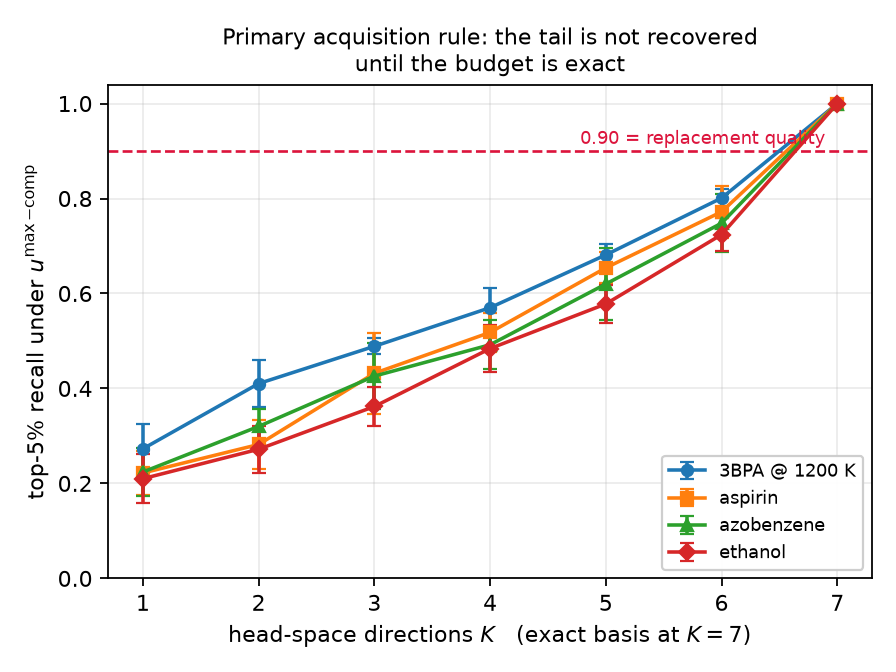
\includegraphics[width=0.52\textwidth]{figures/fig_maxcomp_recall.png}
\caption{The negative result, under the \emph{primary} max-component rule: top-5\% recall against
budget $K$ on all four systems. Recall climbs steadily but never reaches the $0.90$ replacement line
short of the exact basis at $K{=}7$. Error bars are the standard deviation over ten frozen seeds.
Appendix~\ref{app:pareto} plots the corresponding screening Pareto.}
\label{fig:pareto}
\end{figure}

\subsection{Does reducing directions reduce GPU time?}
\label{sec:regime}
Only in some regimes. Against a \emph{batched} exact baseline --- which this stack makes available
only after disabling the TensorExpr fuser (Appendix~\ref{app:tensorexpr}) --- the total
force-plus-UQ speedup at $K{=}3$ is $\fsBestTotalKThreeBSixteen\times$ at $B{=}16$ but collapses to
$\fsBestTotalKThreeBOne\times$ at $B{=}1$, where extra cotangent lanes are nearly free. Appendix~\ref{app:systems} gives the full accounting, the latency table and a kernel profile.

\subsection{Can approximate screening avoid exact computation?}
\label{sec:screening}
This is where the method succeeds --- and, unlike Section~\ref{sec:fidelity}, it succeeds under the
primary max-component rule. With a control variate at $r_0{=}2$, $K{=}4$ and $\alpha{=}0.05$,
evaluated on the held-out test split, with $Q_{r_0}$ and $\tau$ fitted on the design split and
$c_\alpha$ on the calibration split:

\begin{center}\small
\begin{tabular}{lrrr}
\toprule
system & high-UQ recall & exact skipped & screening speedup \\
\midrule
3BPA @ 1200\,K   & \fsGateCVRecallThreeBPA{} \fsGateCVRecallThreeBPACI     & \fsGateCVSkipThreeBPA{} \fsGateCVSkipThreeBPACI     & $\fsGateCVSpeedThreeBPA\times$ \\
rMD17 ethanol    & \fsGateCVRecallEthanol{} \fsGateCVRecallEthanolCI       & \fsGateCVSkipEthanol{} \fsGateCVSkipEthanolCI       & $\fsGateCVSpeedEthanol\times$ \\
rMD17 aspirin    & \fsGateCVRecallAspirin{} \fsGateCVRecallAspirinCI       & \fsGateCVSkipAspirin{} \fsGateCVSkipAspirinCI       & $\fsGateCVSpeedAspirin\times$ \\
rMD17 azobenzene & \fsGateCVRecallAzobenzene{} \fsGateCVRecallAzobenzeneCI & \fsGateCVSkipAzobenzene{} \fsGateCVSkipAzobenzeneCI & $\fsGateCVSpeedAzobenzene\times$ \\
\bottomrule
\end{tabular}
\end{center}

Between $\fsGateCVSkipLo$ and $\fsGateCVSkipHi$ of exact force-UQ evaluations are avoided while
$\fsGateCVRecallLo$--$\fsGateCVRecallHi$ of high-uncertainty configurations are still routed to the
exact computation, on every system. Intervals are $95\%$ paired bootstraps over test structures
(\fsNBoot{} resamples); the positive sets hold only tens of structures, so the recall intervals are
correspondingly wide and we report them rather than the point estimates alone.
The screening gate is where the extreme-value bias of Section~\ref{sec:fidelity} stops mattering:
$c_\alpha$ is a multiplicative calibration constant, so any bias that is monotone in the estimator's
noise is absorbed rather than propagated.

Every gate spends $1{+}K$ lanes per structure and, on fallback, only $r{-}K$ further passes rather
than a fresh $M$ --- charged identically for all gates, since crediting that reuse to one method
alone would manufacture its advantage (Appendix~\ref{app:cost}).

\paragraph{Is the gate doing the work, or is ForceSketch?}
A calibrated gate is a generic wrapper, so the claim only stands if this gate beats the cheaper ones
a reader will reach for. Against a \emph{free} energy-disagreement gate, head subsampling with the
exact mean, and a plain Haar sketch --- all at matched lane budget, identical splits and threshold
--- the control variate \emph{Pareto-dominates} in \fsGateCVDominates{} of \fsGateCVComparisons{}
gate-by-system comparisons. The free gate is the informative failure: its recall collapses to
\fsGateEnergyRecallAzobenzene{} on azobenzene, so energy disagreement is a genuinely different
signal from force disagreement, not a cheap proxy for it. Appendix~\ref{app:gates} gives the full
comparison.

\section{Conclusion and limitations}
\label{sec:limitations}
Exact multi-head force uncertainty cannot be replaced by a handful of randomized head-space probes:
the best sketch reaches only $\fsMaxRecallKFourLo$--$\fsMaxRecallKFourHi$ top-5\% recall at $K{=}4$
and $\fsMaxRecallKSixLo$--$\fsMaxRecallKSixHi$ even at $K{=}6$ of $7$. It can be \emph{screened}:
a split-conformal gate over a control-variate sketch avoids $\fsGateCVSkipLo$--$\fsGateCVSkipHi$ of
exact computations while retaining $\fsGateCVRecallLo$--$\fsGateCVRecallHi$ of high-uncertainty
structures on every system --- a property of the estimator, not the implementation.
\textbf{Limitations.} Whether it saves \emph{time} depends on the regime: at $B{=}1$ extra cotangent
lanes are nearly free, the speedup falls to $\fsBestTotalKThreeBOne\times$ and the gate becomes a net
slowdown, so this suits batched active-learning sweeps, not single-structure MD. We preserve a
\emph{proxy}, not a demonstrated outcome: no active-learning loop is run and no reference-force error
measured, so we claim no gain in model quality or oracle-query efficiency. Committee disagreement is
only a proxy for error; calibration is marginal and under exchangeability; $M{=}8$ bounds the maximum
saving; and rMD17 spans only 9--24 atoms.

\bibliographystyle{plainnat}
\bibliography{references}

\appendix

\section{Screening-gate baselines at matched budget}
\label{app:gates}
\paragraph{Is the gate doing the work, or is ForceSketch?}
A calibrated gate is a generic wrapper --- any score correlated with exact force disagreement can be
calibrated the same way --- so the claim only stands if this gate beats the cheaper ones a reader
will reach for. We build three at matched lane budget with identical splits, calibration and
threshold. The first is \emph{free}: the $M$ head energies come from the forward pass the model
already runs, costing zero \emph{uncertainty} lanes. The second is head subsampling using the
\emph{exact} mean force ForceSketch already pays a lane for,
$\hat v_d=\frac{M}{K(M-1)}\sum_{i\in\mathcal S}(F_{di}-\bar F_d)^2$, unbiased under uniform sampling
and markedly lower-variance than the sample variance among the drawn heads.

\begin{center}\small
\begin{tabular}{lrrrr}
\toprule
gate & lanes & exact skipped & high-UQ recall & speedup \\
\midrule
energy disagreement (free) & $1$ & \fsGateEnergySkipLo--\fsGateEnergySkipHi & \fsGateEnergyRecallLo--\fsGateEnergyRecallHi & $\fsGateEnergySpeedLo$--$\fsGateEnergySpeedHi\times$ \\
head subsampling, exact mean & $5$ & \fsGateHeadExactSkipLo--\fsGateHeadExactSkipHi & \fsGateHeadExactRecallLo--\fsGateHeadExactRecallHi & $\fsGateHeadExactSpeedLo$--$\fsGateHeadExactSpeedHi\times$ \\
Haar sketch & $5$ & \fsGateHaarSkipLo--\fsGateHaarSkipHi & \fsGateHaarRecallLo--\fsGateHaarRecallHi & $\fsGateHaarSpeedLo$--$\fsGateHaarSpeedHi\times$ \\
\textbf{control variate} & $5$ & \textbf{\fsGateCVSkipLo--\fsGateCVSkipHi} & \textbf{\fsGateCVRecallLo--\fsGateCVRecallHi} & $\mathbf{\fsGateCVSpeedLo}$--$\mathbf{\fsGateCVSpeedHi}\mathbf{\times}$ \\
\bottomrule
\end{tabular}
\end{center}

Ranges are across the four systems. The control variate \emph{Pareto-dominates} --- strictly more
skipped \emph{and} strictly higher recall --- in \fsGateCVDominates{} of the \fsGateCVComparisons{}
gate-by-system comparisons, including every one against the two sketch baselines. The exception:
on ethanol the free energy gate attains perfect recall (\fsGateEnergyRecallEthanol{}) while skipping
only \fsGateEnergySkipEthanol. Elsewhere that free gate is the informative failure, collapsing to
\fsGateEnergyRecallAzobenzene{} recall on azobenzene: energy disagreement is a genuinely different
signal from force disagreement, not a cheap proxy for it.


\section{Screening Pareto at matched budget}
\label{app:pareto}
\begin{figure}[h]
\centering
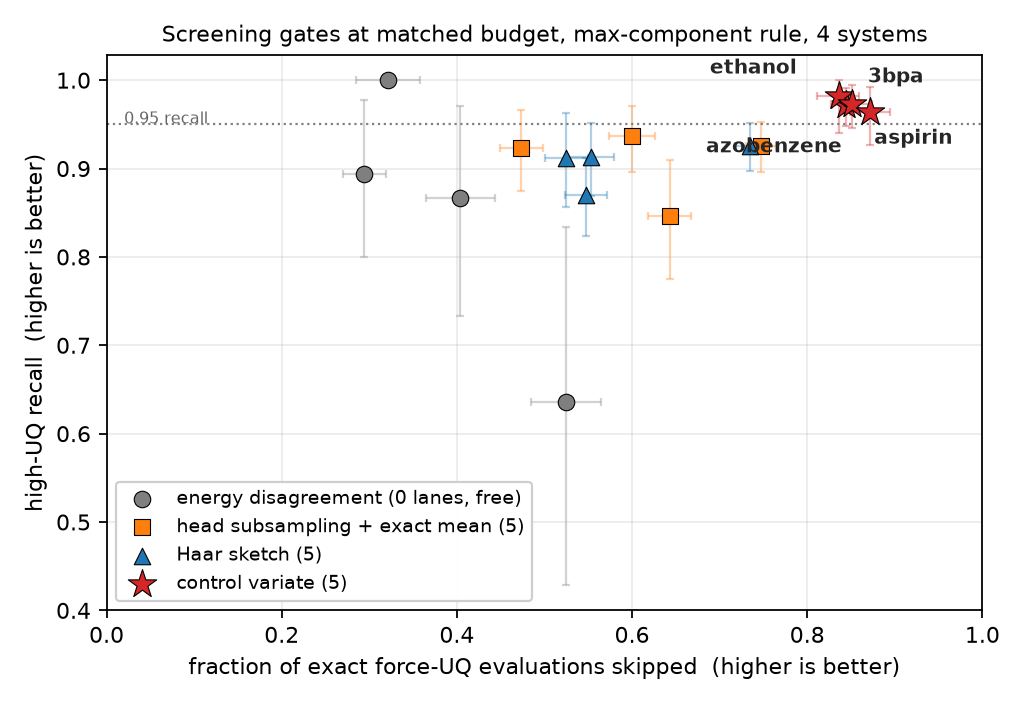
\includegraphics[width=0.6\textwidth]{figures/fig5_gate_pareto.png}
\caption{All four gates at matched lane budget on all four systems, under the max-component rule.
Up-and-right is better on both axes, so the control variate's dominance is read directly. Bars are
$95\%$ paired bootstrap intervals.}
\end{figure}

\section{Data and code availability}
\label{app:avail}
All datasets and model checkpoints used here are public and are pinned by SHA-256 in the artifact's
freeze manifest: the 3BPA~\citep{botnet3bpa} and rMD17~\citep{rmd17} datasets, and the pretrained
multi-head committees released with~\citet{beck2025mhc} (Zenodo record 17829635). The estimator
library, every experiment script, the analysis code, the ten frozen random seeds and every raw
result record behind the numbers in this paper are available at
\url{\fsCodeUrl}. Everything downstream of the cached head-force matrix is offline linear algebra
and reproduces without a GPU; only the timing experiments require one.


\section{Lanes and the centered head subspace}
\label{app:lanes}
\paragraph{Why energies are cheap and forces are not.}
The $M$ energies cost one forward pass because the heads share a trunk. Forces are gradients, and
reverse-mode differentiation returns the gradient of \emph{one scalar} per backward pass. Feeding it
the mean energy yields the mean force, not the spread; feeding it each $E_m$ in turn yields all $M$
force fields but costs $M$ backward passes. We call one backward pass a \emph{lane}.

The saving grace is that $S$ depends on $F$ only through the centered matrix $FP$, whose columns sum
to zero and therefore span at most $M-1$ dimensions. Let $Q\in\mathbb{R}^{M\times(M-1)}$ have
orthonormal columns $q_1,\dots,q_{M-1}$ spanning exactly that centered subspace:
\begin{equation*}
Q^{\mathsf T}Q=I_{M-1},\qquad Q^{\mathsf T}\mathbf 1=0,\qquad QQ^{\mathsf T}=P .
\end{equation*}
Each column is one lane's worth of work. Differentiating the scalar $q_j^{\mathsf T}E$ --- a fixed
weighted combination of the head energies --- costs a single backward pass and returns
\begin{equation}
g_j\;=\;-\nabla_x\bigl(q_j^{\mathsf T}E\bigr)\;=\;Fq_j\;\in\;\mathbb{R}^{D},
\qquad\text{and}\qquad
v_d\;=\;\frac{1}{M-1}\sum_{j=1}^{M-1} g_{j,d}^{\,2} .
\end{equation}
So the exact variance needs $M-1$ lanes, plus one more along the uniform direction
$\tfrac1M\mathbf 1$ for the mean force the simulation needs anyway: $M$ lanes in total, matching the
naive per-head loop. \emph{Our question is whether downstream uncertainty decisions really need all
$M-1$ centered lanes.}


\section{The low-rank control variate}
\label{app:cv}
\paragraph{Low-rank control variate.}
Split $P = Q_{r_0}Q_{r_0}^{\mathsf T} + R$, where $Q_{r_0}\in\mathbb{R}^{M\times r_0}$ has
orthonormal columns inside the centered subspace and $R$ is the projector onto what is left of it,
the \emph{residual} subspace of dimension $r-r_0$. The columns of $Q_{r_0}$ are the $r_0$ leading
eigenvectors of the \emph{design}-split average $\bar A=\tfrac1n\sum_i PF_i^{\mathsf T}F_iP$ --- an
$M\times M$ matrix in \emph{head} space, whose top eigenvector is the weighting of heads along which
this committee disagrees most consistently. It is fitted separately for
each system on structures disjoint from both the calibration and the test splits
(Section~\ref{sec:setup}). Fitting it on the calibration split instead would invalidate the conformal
guarantee below, since split conformal requires the score function --- learned basis included --- to
be frozen before the calibration ratios are formed. The idea is to spend a few lanes where the disagreement actually concentrates, and probe only what
is left over. Evaluate those $r_0$ leading directions exactly, costing $g_j=Fq_j$ for the columns
$q_j$ of $Q_{r_0}$, and sketch only the residual with $K'=K-r_0$ Haar probes drawn inside $R$'s
range, collected as $G\in\mathbb{R}^{D\times K'}$ exactly as before but with the frame now living in
the residual subspace:
\begin{equation}
\widehat v_d \;=\; \frac{1}{r}\Bigl[\textstyle\sum_{j\le r_0} g_{j,d}^{\,2} \;+\; \frac{r-r_0}{K'}\sum_{k=1}^{K'} G_{dk}^{\,2}\Bigr],
\end{equation}
which remains unbiased. By \emph{spectrum} we mean the eigenvalues of $\bar A$ --- how the total
disagreement is divided among head-space directions. The motivation is then the \emph{opposite} of
the intuitive one: a concentrated spectrum does not explain why small $K$ works, it is what
\emph{breaks} a random sketch, since a probe either catches the dominant direction or misses it.


\section{Split-conformal screening}
\label{app:conformal}
\paragraph{Screening rather than replacement.}
If the sketch cannot \emph{replace} the exact score, it can still say when the exact score is
certainly small. Conformal prediction~\citep{vovk2005,crc} turns any score, however crude, into a
calibrated bound using held-out data alone. On a calibration split of $n$ structures disjoint from
design and test, form the ratios $\eta_i=S(x_i)/(\widehat S(x_i)+\epsilon)$, the factor by which
the cheap score underestimates the exact one --- and let $c_\alpha$ be their
$\lceil (n+1)(1-\alpha)\rceil$-th order statistic, large enough to cover all but an $\alpha$
fraction of them. Then $U(x)=c_\alpha\widehat S(x)$ sits above $S(x)$ at least $1-\alpha$ of the
time, so $U(x)<\tau$ \emph{certifies} that the exact score is below the high-uncertainty threshold
$\tau$ too: skip when $U(x)<\tau$, fall back otherwise. Formally this is \emph{marginal} coverage,
$\mathbb P[S(x)\le U(x)]\ge 1-\alpha$, under exchangeability --- not a conditional guarantee and not
an out-of-distribution one. 3BPA at 1200\,K calibrated against 300\,K behaviour is exactly such a
shift, so we report the observed coverage there rather than assume it.


\section{The acquisition decision and the extreme-value bias}
\label{app:acq}
\paragraph{The acquisition decision, stated exactly.}
\label{par:acq}
Every number below concerns one decision: from a pool of held-out structures, select the most
force-uncertain fraction for exact reference computation. Following \citet{beck2025mhc}, structures
are ranked by the maximum disagreement of their force components; we evaluate that extreme-value
rule in both of its defensible forms --- maximum over components, maximum over atoms --- and report
the global sum as an easier diagnostic statistic:
\begin{equation}
\widehat u^{\max\text{-comp}}(x)=\max_{d}\widehat\sigma_d,\qquad
\widehat u^{\max\text{-atom}}(x)=\max_{a}\widehat u_a^{\mathrm{MHC}},\qquad
\widehat S(x)=\sum_{d}\widehat v_d .
\end{equation}
A hat always denotes the sketched estimate of the corresponding exact quantity: the exact scores are
the same three expressions with $v_d$ and $\sigma_d=\sqrt{v_d}$ in place of $\widehat v_d$ and
$\widehat\sigma_d$, so the exact $S$ here is exactly the $S$ of Eq.~(1). The correction $c$ is
$c_K$ for Gaussian probes and $c^{\mathrm{Haar}}_{K,r}$ for orthogonal ones
(Section~\ref{sec:method}); $u_a^{\mathrm{MHC}}$ is as in Section~\ref{sec:problem}. We take
$u^{\max\text{-comp}}$ as primary, being the most literal reading, report $u^{\max\text{-atom}}$
alongside it in the artifact, and treat $S$ as the statistically \emph{easier} secondary: a sum over
$3N$ coordinates concentrates, whereas both maxima are extreme-value statistics of a noisy
$\widehat\sigma$.

The two experiments select positives differently and we do not conflate them.
Section~\ref{sec:fidelity} measures \textbf{top-5\% recall}: the $5\%$ of evaluated structures with
the largest \emph{exact} score, ties resolved inclusively, so the set may slightly exceed $5\%$.
Section~\ref{sec:screening} applies a \emph{fixed} threshold instead, as a deployed gate must:
$\tau$ is the $95$th percentile of the exact score on the design split, and a test structure counts
as high-uncertainty when its exact score is at least $\tau$ --- so the realised test prevalence is
$\fsTestPrevalenceLo$--$\fsTestPrevalenceHi$, not exactly $0.05$. Every metric is computed
\emph{per seed and then averaged} over the ten frozen seeds: the deployed budget is $K$ lanes, not
$10K$, and averaging the sketches before scoring would be a different, far more accurate estimator
than the one we claim.


\paragraph{Why the extreme-value rule is harder.}
Making each $\widehat\sigma_d$ unbiased \emph{marginally} is not the same as making
$\max_d\widehat\sigma_d$ unbiased: a maximum over $3N$ noisy estimates is biased upward, and the
bias grows with the estimator's noise. Measured directly, $u^{\max\text{-comp}}$ is inflated by
$\fsMaxBiasKOneLo$--$\fsMaxBiasKOneHi$ at $K{=}1$, falling to
$\fsMaxBiasKFourLo$--$\fsMaxBiasKFourHi$ at $K{=}4$ and to \fsMaxBiasExact{} at the full basis,
where the estimator is exact and the bias must vanish --- a useful check on the pipeline. This
obstructs \emph{replacement} but not screening (Section~\ref{sec:screening}): the bias is monotone
in the estimator's noise, so a scale-calibrated gate absorbs it into $c_\alpha$.

Orthogonalizing the probes is the largest single lever in the method. The estimator comparisons that
follow are on the global statistic, where the paired-bootstrap machinery of Section~\ref{sec:setup}
was frozen; the ordering they establish is a property of the estimators, not of the acquisition rule.
The paired difference between Haar and Gaussian at $K{=}3$, evaluated on identical structure
resamples, is
$\fsDeltaOrtho$ \fsDeltaOrthoCI{} in top-5\% recall, and is significant on all four systems. The
low-rank control variate adds a further $\fsDeltaCV$ \fsDeltaCVCI{} over Haar at $K{=}4$, reaching
\fsCVRecallKFour{} \fsCVRecallKFourCI{} --- still short of 0.90.

The head-space spectrum explains why. Writing $A=\bar{Q^{\mathsf T}F^{\mathsf T}FQ}$ for the averaged
centered force-disagreement Gram matrix, the stable rank of the matrix we actually sketch is
$\operatorname{srank}(FQ)=\|FQ\|_F^2/\|FQ\|_2^2=\operatorname{tr}(A)/\lambda_{\max}
=\fsSrankLo$--$\fsSrankHi$ of a maximum $7$ across the four systems, with the leading direction
carrying $\fsTopEigLo$--$\fsTopEigHi$ of the disagreement (an isotropic spectrum would give
$\fsTopEigIsotropic$). The spectrum is therefore \emph{moderately diffuse rather than strongly
rank-concentrated} --- but far from isotropic, at
$\fsTopEigRatioLo$--$\fsTopEigRatioHi\times$ the isotropic leading share.
That is exactly the regime in which a random $K$-dimensional projection pays a variance penalty, and
it is why projecting out the leading directions (the control variate) recovers so much.



\section{What ForceSketch replaces}
\label{app:schematic}
\begin{figure}[t]
\centering
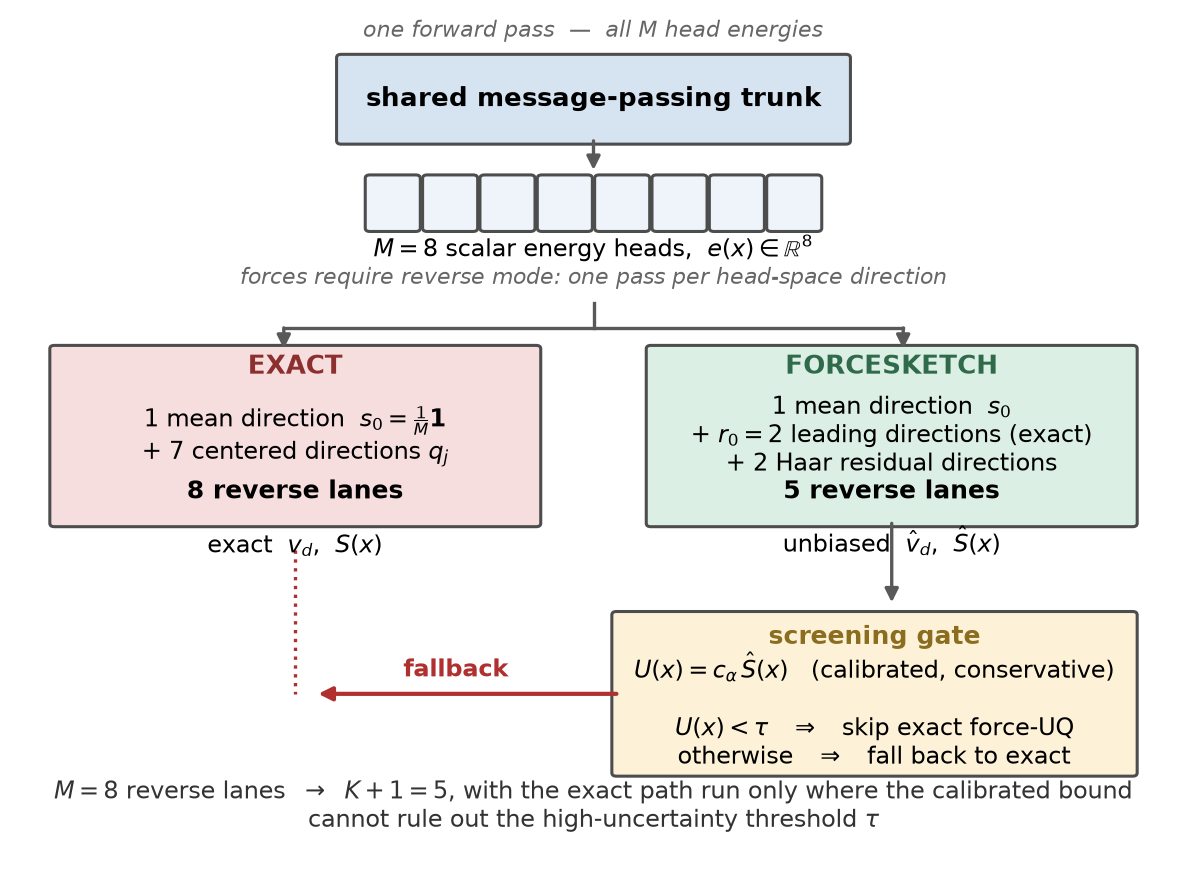
\includegraphics[width=0.68\textwidth]{figures/fig1_schematic.png}
\caption{What ForceSketch replaces. All $M$ head energies come from one forward pass, but forces do
not: exact disagreement needs the full centered head subspace, $M$ lanes. ForceSketch spends $K{+}1$,
and --- since that is not accurate enough to \emph{replace} exact uncertainty at $K\le4$ under either
acquisition rule (Section~\ref{sec:fidelity}) --- its score feeds a calibrated gate that runs the
exact path only where the bound cannot rule out the threshold. Whether fewer lanes also cost less
time depends on the autodiff regime (Section~\ref{sec:regime}).}
\label{fig:schematic}
\end{figure}


\section{Finite-$K$ corrections}
\label{app:finitek}
\paragraph{Finite-$K$ corrections.}
Reporting a standard deviation means taking a square root, and the square root of an unbiased
variance estimate is \emph{not} an unbiased standard-deviation estimate: $\sqrt{\cdot}$ is concave,
so $\sqrt{\widehat v_d}$ is biased low, the more so the fewer probes we spend. The fix is a
multiplicative constant depending only on $K$ (and, for orthogonal probes, on $r$).
For Gaussian probes $K\widehat v_d/v_d\sim\chi^2_K$ and the
correction is $c_K=\sqrt{2/K}\,\Gamma(\tfrac{K+1}{2})/\Gamma(\tfrac K2)$. For Haar probes the
analogous constant is conventionally written with Beta functions, which is singular at $K=r$
(it evaluates $B(K/2,0)$). Cancelling the shared $\Gamma(\tfrac{r-K}{2})$ gives a form that is
finite everywhere and exactly $1$ at full rank:
\begin{equation}
c^{\mathrm{Haar}}_{K,r}\;=\;\sqrt{\tfrac{r}{K}}\;
\frac{\Gamma\!\left(\tfrac{K+1}{2}\right)\Gamma\!\left(\tfrac r2\right)}
     {\Gamma\!\left(\tfrac K2\right)\Gamma\!\left(\tfrac{r+1}{2}\right)} ,
\qquad c^{\mathrm{Haar}}_{K,r}\to c_K \ \text{ as } r\to\infty .
\end{equation}
We verify unbiasedness of $\sqrt{\widehat v}/c$ to within Monte-Carlo error at $4\times10^5$ draws.
These closed forms cover the Gaussian and Haar estimators; the control variate below mixes exact and
sketched directions and has no such constant, so we apply the residual frame's Haar correction,
which is an approximation. It does not affect the screening results, because $c_\alpha$ is itself a
multiplicative calibration and absorbs any constant scale error exactly.


\section{Splits}
\label{app:splits}
\paragraph{Splits.}
Each system is partitioned once, under a frozen permutation, into three disjoint splits: a
\emph{design} split ($20\%$) fitting the control-variate basis $Q_{r_0}$ and the threshold $\tau$; a
\emph{calibration} split ($20\%$) fitting the conformal constant $c_\alpha$ alone; and a \emph{test}
split ($60\%$), touched once --- $\fsNDesignThreeBPA/\fsNCalThreeBPA/\fsNTestThreeBPA$ structures for
3BPA and $\fsNDesignEthanol/\fsNCalEthanol/\fsNTestEthanol$ per rMD17 molecule. The separation is not
cosmetic: split-conformal coverage requires the score function to be frozen independently of the
calibration observations, so a basis fitted on calibration structures would void the guarantee. The
code asserts all three pairwise disjointness conditions and that the splits partition the set.


\section{Does reducing directions reduce GPU time?}
\label{app:systems}
\subsection{Does reducing directions reduce GPU time?}
\label{sec:regime}
Only in some regimes, and the honest answer required first making the strongest baseline available.
Batched reverse mode --- vectorizing the backward over cotangents while reusing one forward graph ---
is the baseline fairness demands, and on this stack it fails from the third call onwards, which
disguises the cause. Appendix~\ref{app:tensorexpr} diagnoses it (the TensorExpr fuser and e3nn's
scripted spherical harmonics~\citep{e3nn}); Appendix~\ref{app:compile} shows
that compilation does not compose with it; without the fix we would have compared against a Python
loop and overstated every speedup below.

Two ratios answer different questions and we never conflate them. With $T(L)$ the latency of an
$L$-lane reverse pass, the \emph{incremental UQ} speedup $[T(M)-T(1)]/[T(1{+}K)-T(1)]$ is the cost
of uncertainty once the mean force is paid for, while the \emph{total force-plus-UQ} speedup
$T(M)/T(1{+}K)$ includes it. We lead with the total, because the incremental ratio is unstable at
small batch precisely when $T(1{+}K)\approx T(1)$ --- which is the effect this section is about.

That effect is large. Batched reverse mode is nearly \emph{flat} in the lane count at $B{=}1$
($\fsBatchedFlatLaneOne$\,ms for one lane, $\fsBatchedFlatLaneEight$\,ms for eight), so extra
cotangents are almost free and the total speedup at $K{=}3$ collapses to
$\fsBestTotalKThreeBOne\times$ --- against $\fsSerialTotalKThreeBOne\times$ if one compares only to a
serial loop. At $B{=}16$ the batched path scales with $L$ again and the speedup recovers to
$\fsBestTotalKThreeBSixteen\times$; by $B{=}\fsBatchedLosesBatch{}$ it is slower than the serial loop
at \emph{every} lane count measured ($\fsBatchedRatioLost\times$ at $L{=}8$), so serial becomes the
strongest baseline again and the speedup is $\fsSerialTotalKThreeBSixtyFour\times$. Incremental
speedups are $\fsBestIncrKThreeBOne\times$ and $\fsBestIncrKThreeBSixteen\times$ at $B{=}1$ and
$B{=}16$. Appendix~\ref{app:latency} tabulates the latencies behind these ratios and
Appendix~\ref{app:kernels} profiles where the GPU time goes.


\section{What a screened evaluation costs}
\label{app:cost}
\paragraph{What a screened evaluation costs.}
Every gate spends $1{+}K$ lanes per structure: one mean-force lane, which MD needs regardless, plus
$K$ uncertainty lanes. On fallback it does \emph{not} restart: the $K$ directions already evaluated
are linearly independent inside the $r$-dimensional centered subspace, and an orthonormal frame
spanning them is a recombination of vectors already in hand, so completing the exact basis costs
only $r{-}K$ further passes. With $p$ the fallback fraction,
$T_{\mathrm{screen}}=T(1{+}K)+p\,T(r{-}K)$ against $T_{\mathrm{exact}}=T(M)$ --- at $K{=}4$, $M{=}8$,
$T(5)+p\,T(\fsFallbackLanesSketch)$, while the free energy gate, evaluating no centered direction,
pays $T(1)+p\,T(\fsFallbackLanesEnergy)$. Crediting that reuse to the control variate alone would
manufacture much of its advantage, so every gate is charged this way. $T(\cdot)$ is the measured
median at $B{=}16$ under whichever implementation is faster at that lane count
(Section~\ref{sec:regime}); fallback is charged a fresh forward rather than a retained graph, which
is conservative; and the quoted figure is the \emph{total} force-plus-UQ speedup.


\section{Diagnosing the batched reverse-mode failure}
\label{app:tensorexpr}
\paragraph{Batched reverse mode, and why it initially appeared impossible.}
\texttt{torch.autograd.grad(is\_grads\_batched=True)} vectorizes the backward over cotangents while
reusing one forward graph, and is the baseline spec-level fairness demands. On this stack it fails
with \texttt{Cannot access data pointer of Tensor that doesn't have storage} --- but only from the
third call onwards, which disguises the cause. The mechanism is: batched reverse mode runs under
\texttt{torch.\_vmap\_internals}, so cotangents are \texttt{BatchedTensor}s with no storage;
TorchScript's profiling executor emits an optimized plan only after two warm-ups; and the TensorExpr
fuser then fuses the \emph{reverse} graph into a \texttt{prim::TensorExprGroup}, whose kernel
requires a raw \texttt{data\_ptr()} for every input. The TorchScript on the path is
\texttt{e3nn}'s \texttt{\_spherical\_harmonics}, a module-level \texttt{@torch.jit.script}
\emph{free function} --- not a module, so walking the module tree finds nothing to un-script, and a
fully rebuilt zero-\texttt{ScriptModule} model still fails. Disabling the TensorExpr fuser before
the first forward fixes it: 50/50 consecutive batched calls agreeing with the serial path to
$3\times10^{-15}$, at a $\sim\!4\%$ cost to the serial path from losing fusion. We report this
because it is a trap any e3nn-based UQ work will hit, and because without it we would have compared
against a Python loop, which spec-level fairness forbids.


\section{Accuracy and cost on the global statistic}
\label{app:ktradeoff}
Figure~\ref{fig:pareto} (left) plots recall against $K$ under the primary max-component rule. For
completeness the same trade-off on the easier global statistic $S$, together with the latency curve,
is below; it is the secondary view, and is uniformly more optimistic.

\begin{figure}[t]
\centering
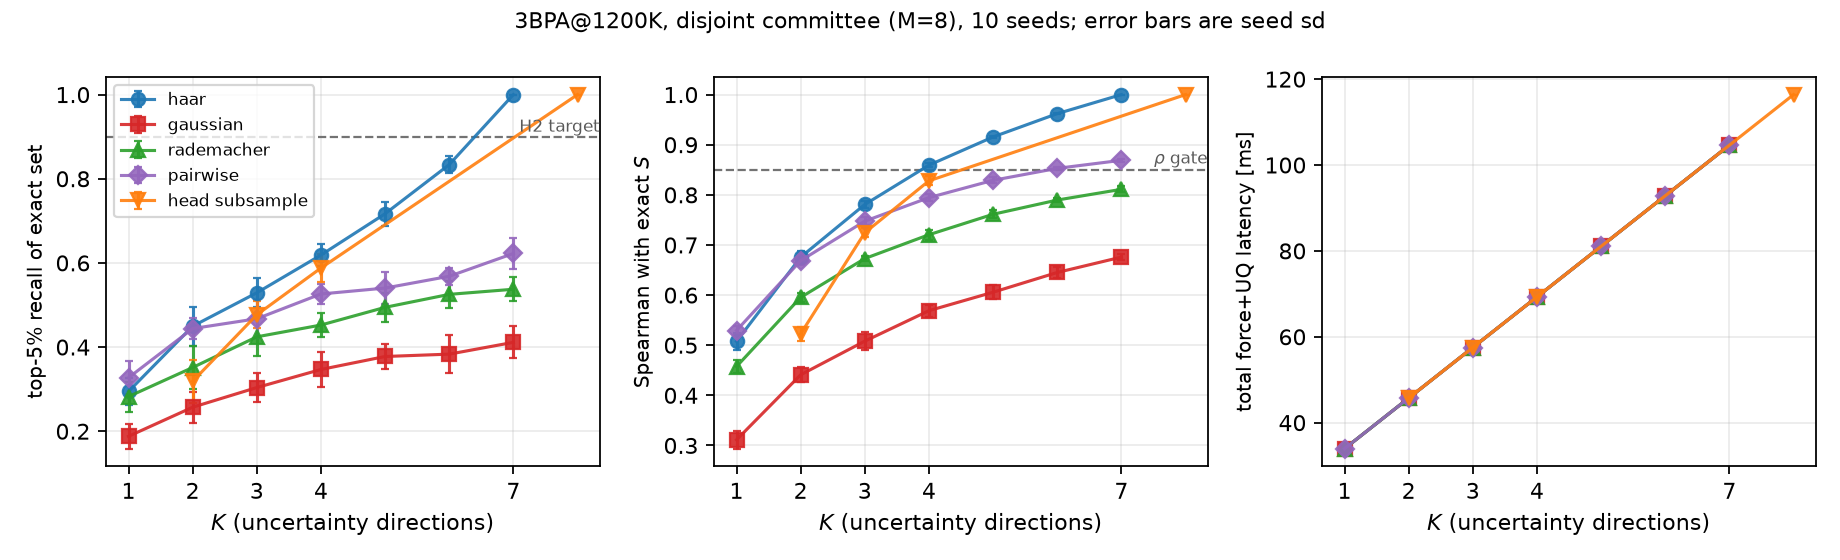
\includegraphics[width=0.92\textwidth]{figures/fig3_k_tradeoff.png}
\caption{Accuracy and cost against $K$, ranked by the global statistic $S$. Latency curves coincide
for every method at equal lane count under the serial implementation; batched reverse mode flattens
them (Section~\ref{sec:regime}). Ranking saturates well before tail selection: Haar clears Spearman
$\rho=0.85$ at $K{=}4$ while its top-5\% recall is still $\fsHaarRecallKFour$. Error bars are the
standard deviation across the ten frozen seeds.}
\label{fig:ktradeoff}
\end{figure}

\section{Measured serial and batched latency}
\label{app:latency}
\begin{center}\small
% Generated by analysis/tables.py -- do not edit by hand.
\begin{tabular}{rrrrr}
\toprule
 & \multicolumn{2}{c}{$B=1$ (27 atoms)} & \multicolumn{2}{c}{$B=16$ (432 atoms)} \\
lanes $L$ & serial & batched & serial & batched \\
\midrule
1 & \textbf{22.9} & 25.5 & \textbf{24.3} & 26.0 \\
4 & 60.3 & \textbf{27.5} & 62.5 & \textbf{39.7} \\
8 & 110.5 & \textbf{30.5} & 115.5 & \textbf{73.2} \\
\bottomrule
\end{tabular}

\end{center}
\vspace{-0.4em}
{\small Median latency in ms, fp32, one RTX 5070 Laptop GPU, CUDA events with one event pair per
iteration; \textbf{bold} marks the faster implementation at that $(B,L)$. These are the measurements
behind every speedup quoted in Section~\ref{sec:regime}.}

\section{Compilation, and why it does not compose}
\label{app:compile}
For completeness we also compiled the model. \texttt{torch.compile}~\citep{torchcompile} succeeds only partially here ---
Dynamo builds a sequence-length guard on e3nn's \texttt{Irrep} and calls \texttt{len()} on it, which
e3nn raises \texttt{NotImplementedError} for by design, so untraceable regions must fall back to
eager. With that, compilation is correct to $\fsCompileRelErr$ and gives
$\fsCompileSpeedupLo$--$\fsCompileSpeedupHi\times$ at $B{=}16$. The absolute saving grows linearly in
$L$, so AOTAutograd is producing a cheaper backward rather than merely a faster forward.

The obvious next question is whether the two accelerations \emph{compose}: compiled-plus-batched
would then be the baseline fairness demands. They do not. With the TensorExpr fuser already disabled,
compiling the model and then taking a batched VJP reproduces the identical
\texttt{Cannot access data pointer of Tensor that doesn't have storage} failure, at both $B{=}1$ and
$B{=}16$ --- AOTAutograd's compiled backward is no more able to accept a storage-free
\texttt{BatchedTensor} than the fused TorchScript one was. We therefore report the eager batched
path as primary because it is the fastest \emph{correct} baseline available on this stack, not
merely the most convenient one, and note that compilation alone would shift these numbers by at most
a few percent in the same direction for every method, leaving the crossover of
Section~\ref{sec:regime} unchanged.

\section{Where the GPU time goes}
\label{app:kernels}
A kernel-level profile of the serial path explains why removing lanes helps at all when it does: the
composition of GPU time is invariant in $L$ (elementwise $\fsKernElemExact\%$ at $L{=}7$ against
$\fsKernElemSketchLo$--$\fsKernElemSketchHi\%$ at $L{=}2,3,4$; tensor products
$\fsKernTPExact\%$ against $\fsKernTPSketchLo$--$\fsKernTPSketchHi\%$; the same \fsKernDistinct{}
distinct kernels throughout), and only the repetition count changes: kernel launches fall by
$\fsKernLaunchRatio\times$ from the exact path to $K{=}3$, against a lane ratio of
$\fsKernLaneRatio\times$. Sketching linearly reduces repeated execution of the shared trunk, and
batched reverse mode attacks the same redundancy by a different route --- which is exactly why the
two are substitutive at small batch.

\section{Sketching versus using fewer heads}
\label{app:headsub}
At equal total lanes, does a random sketch beat simply computing a few of the head forces exactly?
The comparison hinges on which head-subsampling estimator is used, and the fair one is not the
obvious one. Bare head subsampling takes the sample variance among the $K$ drawn heads. But at
matched budget it also pays a mean-force lane, and can therefore use the \emph{exact} mean:
\begin{equation*}
\widehat v^{\,\text{sub}}_d \;=\; \frac{M}{K(M-1)}\sum_{i\in\mathcal S}\bigl(F_{di}-\bar F_d\bigr)^2 ,
\end{equation*}
unbiased under uniform sampling without replacement and markedly lower-variance than the sample
variance, because it does not spend degrees of freedom re-estimating a mean already in hand.

Against that fair baseline the ordering \emph{reverses}. Haar at $K{=}3$ scores
$\fsDeltaVsHeadSub$ \fsDeltaVsHeadSubCI{} against exact-mean head subsampling at $K{=}3$ on 3BPA and
$\fsDeltaVsHeadSubAspirin$ \fsDeltaVsHeadSubAspirinCI{} on aspirin --- both significantly
\emph{negative}, i.e.\ head subsampling wins --- and the difference is not significant on ethanol or
azobenzene. An earlier version of this comparison scored the baseline with the sample variance while
still charging it the mean lane, and reported Haar ahead; that was an artifact of hobbling the
baseline, and we report the corrected result instead. Head subsampling at $K{=}4$ with no mean lane
also beats Haar at equal lanes ($\fsDeltaVsHeadSubNoMeanThreeBPA$
\fsDeltaVsHeadSubNoMeanThreeBPACI{} on 3BPA), but cannot produce the mean force MD requires.

The paper's estimator-design claims do not rest on this comparison. Orthogonalization over Gaussian
probes ($\fsDeltaOrtho$ \fsDeltaOrthoCI{}, significant on all four systems) and the control variate
over Haar ($\fsDeltaCV$ \fsDeltaCVCI{}) are unaffected, and it is the control variate --- not the
oblivious sketch --- that wins the screening comparison of Section~\ref{sec:screening}, where
exact-mean head subsampling is included as a gate baseline in its fair form.

\section*{Submission Checklist}

\begin{enumerate}

\item {\bf Claims}
    \item[] Question: Do the main claims in the abstract and introduction accurately reflect the paper's contributions and scope?
    \item[] Answer: \answerYes{}
    \item[] Justification: The abstract leads with the negative result (at $K\le4$ no estimator recovers the exact top-5\% set) and confines the positive claim to screening. It also gives the batch size at which the wall-clock benefit disappears.

\item {\bf Limitations}
    \item[] Question: Does the paper discuss the limitations of the work?
    \item[] Answer: \answerYes{}
    \item[] Justification: Section~\ref{sec:limitations} gives them: the gate is a net slowdown at batch size~1, the batched-versus-serial crossover is specific to our 8\,GB GPU, calibration is marginal and under exchangeability, and committee disagreement is only a proxy for error. We also say there that we ran no active-learning loop.

\item {\bf AI / LLM disclosure} \emph{(important)}
    \item[] Question: Does the paper disclose any use of AI/LLMs in the research or writing (e.g., ideation, code generation, data processing, drafting), in line with the NeurIPS LLM policy?
    \item[] Answer: \answerYes{}
    \item[] Justification: Claude was used throughout: writing the estimator library and analysis code, running the experiments, and drafting the manuscript. The author set the research question and the experimental design, checked the results against the raw records, and is responsible for the content.

\item {\bf Research integrity \& originality}
    \item[] Question: Do you confirm that this is an original submission --- not a duplicate or lightly tweaked resubmission, nor one of multiple versions of the same work submitted to this workshop --- and that you comply with research-integrity guidelines?
    \item[] Answer: \answerYes{}
    \item[] Justification: Original work, submitted once here, and not a reworked version of an earlier submission. It may be under review concurrently at another non-archival workshop, which this call for papers permits.

\item {\bf Reproducibility} \emph{(optional)}
    \item[] Question: Where applicable, does the paper provide enough information (data, code, settings) to reproduce the main results?
    \item[] Answer: \answerYes{}
    \item[] Justification: Datasets, checkpoints, the environment lockfile and the ten random seeds are pinned by SHA-256 in the artifact's freeze manifest; the code and every raw result record are at \url{\fsCodeUrl}. Confidence intervals are paired bootstraps over structures with $10^4$ resamples.

\end{enumerate}


\end{document}
